\section{Results}\label{sec:ResFit:Results}

The measured Gaussian resolutions, corrected for the effects of
additional jets and out-of-cone showering, are shown for different
\ptref in \qsubfig{fig:ResFit:ResoGauss}{left} for simulated
data.
Here, the \ptref are the mean values of the asssumed spectra~$f(\pttrue)$
in each \ptave bin (comp. \qsubfig{fig:ResFit:Asym:Spectrum}{right}).
The error bars represent the statistical uncertainty from the
extrapolation procedure only (comp. the corresponding remarks in
\qsec{sec:ResFit:AddJets:Extrapolation}).
The measured resolutions are compared to the MC truth resolution.
The latter has been derived from Gaussian fits to the bulk of the
\mbox{$\pt / \ptgen$} distributions of the leading two generator
level jets in an event in small bins of \ptgen, where the
detector level jets are required to match the generator level jets
within a distance of $0.2$ in \mbox{$(\eta,\phi)$} space.
There is good closure of the presented method.

The corresponding measurement in Collider data is shown in \qsubfig{fig:ResFit:ResoGauss}{right}.
The jet \pt resolution is underestimated by about $10\%$ in the MC simulation.

\begin{figure}[ht]
  \label{fig:ResFit:ResoGauss}
  \centering
  \begin{tabular}{cc}
    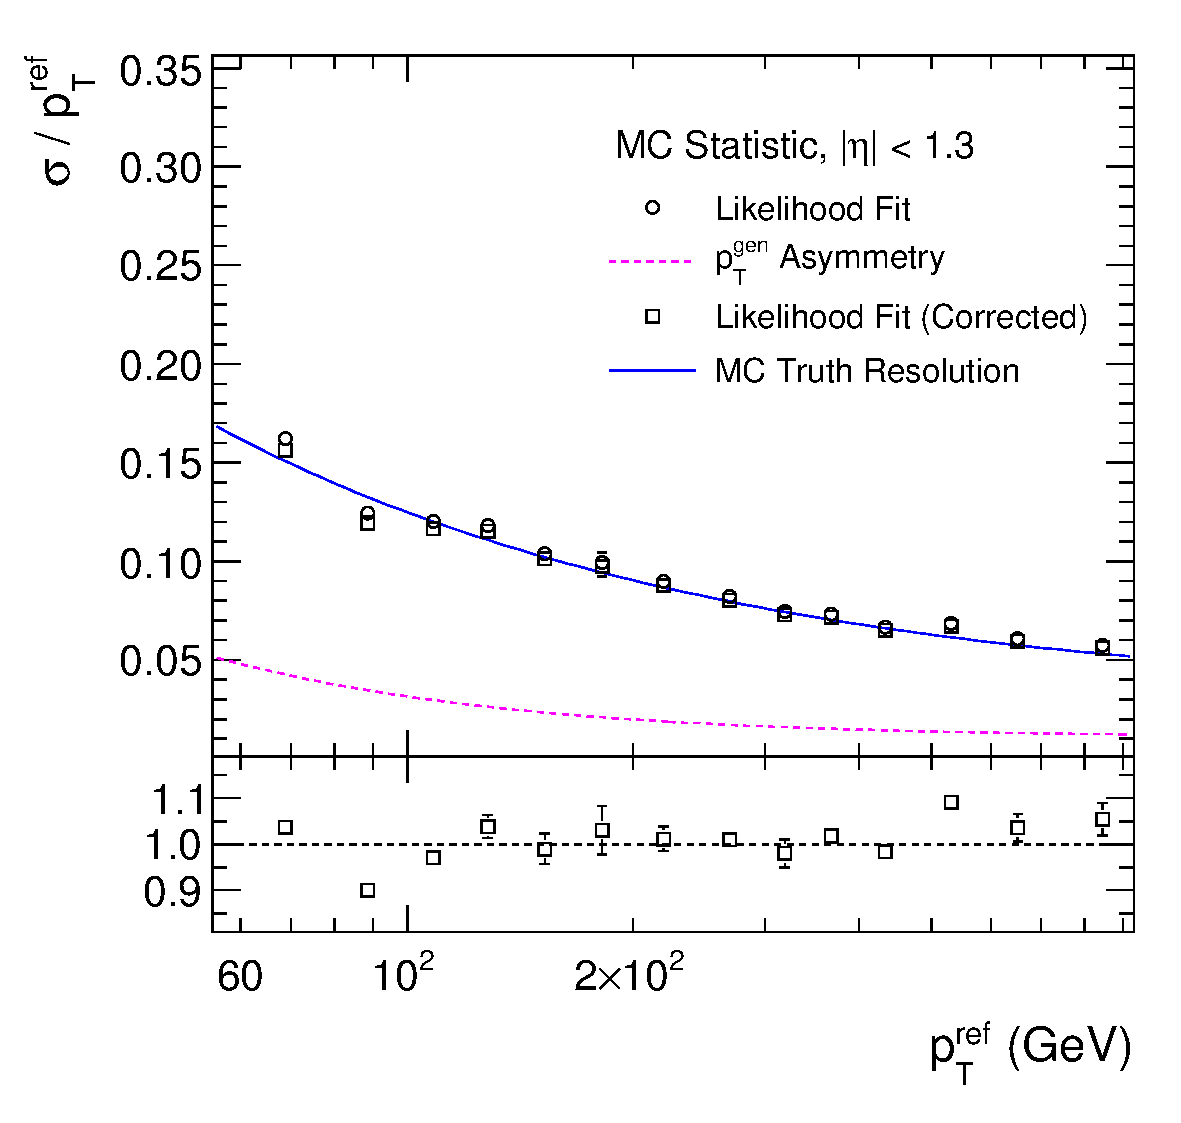
\includegraphics[width=0.45\textwidth]{figures/MaxLike_Eta00-13_ExtraResoBottomRatio}
    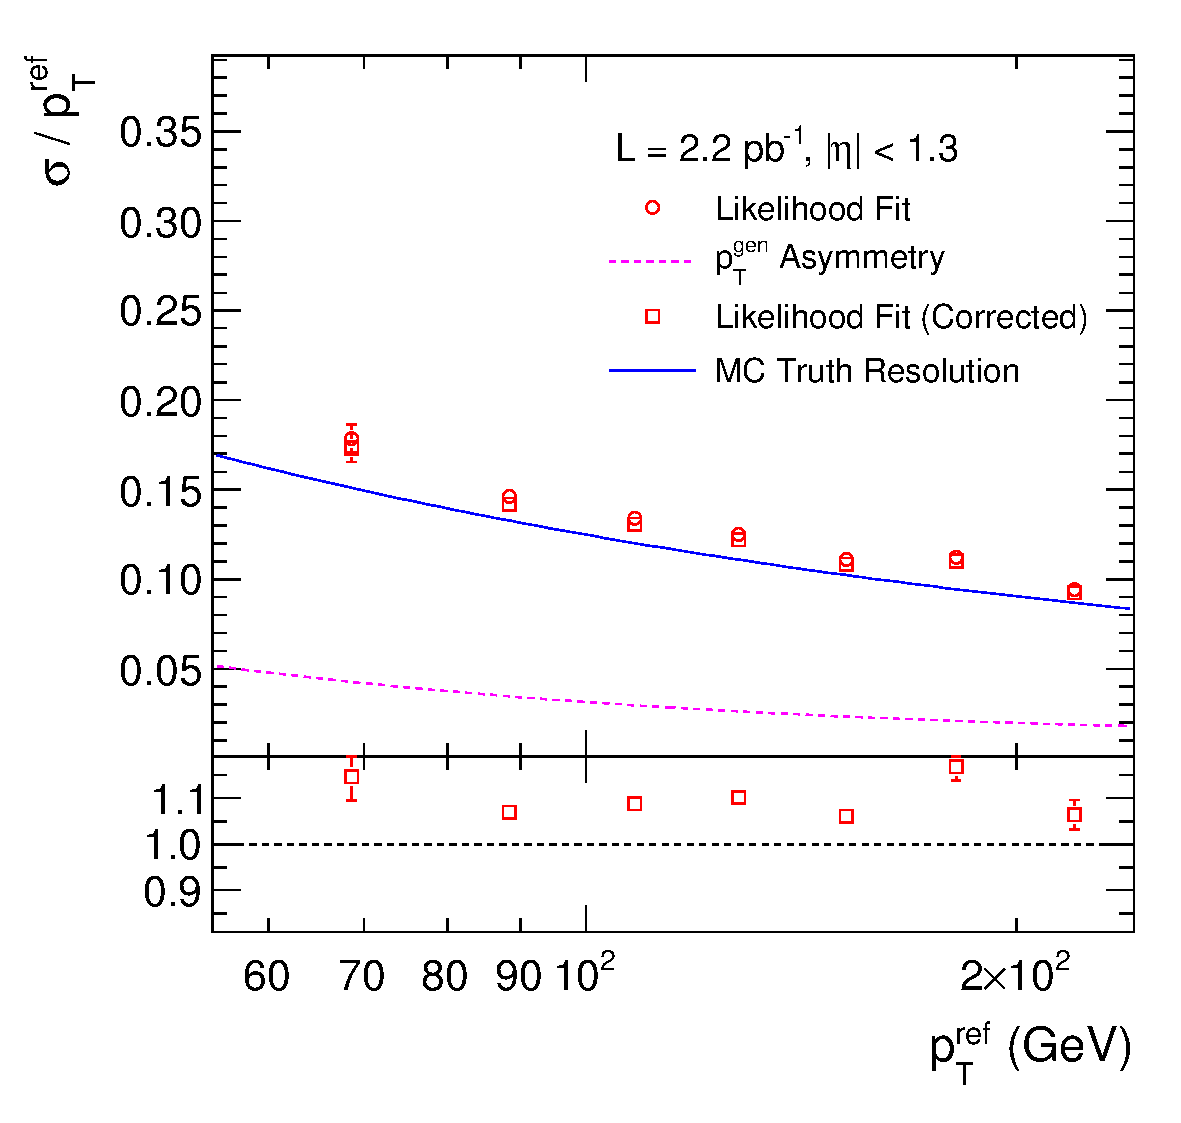
\includegraphics[width=0.45\textwidth]{figures/MaxLike_Data132440-144011_Eta00-13_ExtraResoBottomRatio}\\
  \end{tabular}
  \caption{Measured Gaussian resolutions corrected for
    contributions from additional jets (circles) in different \pt bins.
    Out-of-cone contributions (dashed line) are substracted in
    quadrature to obtain the final resolution (squares).
    The \ptref are the mean values of the asssumed spectra~$f(\pttrue)$
    in each bin (comp. Fig.~\ref{fig:qcd:resolMaxlike:ptGenSpectra}
    (right)).
    (\textit{Left}) Measured resolution in simulated data; there is good
    agreement to the MC truth resolutioin (solid line).
    (\textit{Right}) Measured resolution in Collider data; it is
    $\approx10\%$ larger than the simulation.
  }
\end{figure}
